\documentclass[]{elsarticle} %review=doublespace preprint=single 5p=2 column
%%% Begin My package additions %%%%%%%%%%%%%%%%%%%
\usepackage[hyphens]{url}



\usepackage{lineno} % add
\providecommand{\tightlist}{%
  \setlength{\itemsep}{0pt}\setlength{\parskip}{0pt}}

\usepackage{graphicx}
%%%%%%%%%%%%%%%% end my additions to header

\usepackage[T1]{fontenc}
\usepackage{lmodern}
\usepackage{amssymb,amsmath}
\usepackage{ifxetex,ifluatex}
\usepackage{fixltx2e} % provides \textsubscript
% use upquote if available, for straight quotes in verbatim environments
\IfFileExists{upquote.sty}{\usepackage{upquote}}{}
\ifnum 0\ifxetex 1\fi\ifluatex 1\fi=0 % if pdftex
  \usepackage[utf8]{inputenc}
\else % if luatex or xelatex
  \usepackage{fontspec}
  \ifxetex
    \usepackage{xltxtra,xunicode}
  \fi
  \defaultfontfeatures{Mapping=tex-text,Scale=MatchLowercase}
  \newcommand{\euro}{€}
\fi
% use microtype if available
\IfFileExists{microtype.sty}{\usepackage{microtype}}{}
\bibliographystyle{elsarticle-harv}
\usepackage{longtable,booktabs,array}
\usepackage{calc} % for calculating minipage widths
% Correct order of tables after \paragraph or \subparagraph
\usepackage{etoolbox}
\makeatletter
\patchcmd\longtable{\par}{\if@noskipsec\mbox{}\fi\par}{}{}
\makeatother
% Allow footnotes in longtable head/foot
\IfFileExists{footnotehyper.sty}{\usepackage{footnotehyper}}{\usepackage{footnote}}
\makesavenoteenv{longtable}
\ifxetex
  \usepackage[setpagesize=false, % page size defined by xetex
              unicode=false, % unicode breaks when used with xetex
              xetex]{hyperref}
\else
  \usepackage[unicode=true]{hyperref}
\fi
\hypersetup{breaklinks=true,
            bookmarks=true,
            pdfauthor={},
            pdftitle={A linear mixed effects model of UAP sightings},
            colorlinks=false,
            urlcolor=blue,
            linkcolor=magenta,
            pdfborder={0 0 0}}
\urlstyle{same}  % don't use monospace font for urls

\setcounter{secnumdepth}{0}
% Pandoc toggle for numbering sections (defaults to be off)
\setcounter{secnumdepth}{0}

% Pandoc citation processing

% Pandoc header



\begin{document}
\begin{frontmatter}

  \title{A linear mixed effects model of UAP sightings}
    \author[]{Benjamin Horvath\corref{1}}
  
        \cortext[1]{Data scientist, Brooklyn, NY. E-mail:
\texttt{benhorvath@gmail.com}. Replication files:
\texttt{https://github.com/benhorvath/nuforc\_stats/}.}
  
  \begin{abstract}
  Unidentified aeriel phenomena (UAP) have only recently captured the
  interest of the U.S. Congress, though there is a long history of
  attempting to elucidate the phenomena via the scientific method. The
  natural first step is to plot reported sightings on a map to locate
  potential `hot spots.' However, maps of UAP sightings merely reflect
  population distribution. That is, the biggest clusters coincide with
  the biggest populations. This is not informative. This paper uses
  mixed effects linear regression to quantify the effect of population
  and land area on U.S. counties' reported UAP from 2010--2020. The
  model errors are then interpreted as the number of sightings in excess
  of the pure population/area effect. This generates a list of `true'
  potential hot spots, which include the counties around Myrtle Beach,
  SC; Phoenix, AZ; and Seattle, WA. Further investigation of these
  locales may generate novel hypotheses to be tested or placements for
  electronic sensor systems.
  \end{abstract}
  
 \end{frontmatter}

\hypertarget{introduction}{%
\section{Introduction}\label{introduction}}

A December 2017 story in the \emph{New York Times} revealed the
existence of a secret U.S. military program studying `advanced aerospace
threats' (Cooper, Blumenthal, and Kean 2017). Concerned pilots and other
military personnel reported observing strange aircraft with astounding
capabilities. The Pentagon labeled these objects \emph{unidentified
aerial phenomena} (UAP), though they are more widely known as
unidentified flying objects (UFOs). These reports aroused such concern
in military and political circles that Congress ordered the intelligence
community to prepare a comprehensive report on UAP (ODNI 2021).

These incidents also catalyzed a number of non-governmental projects to
scientifically study UAP. The Galileo Project is perhaps the most
notable, consisting of team of academics assembled by the famed Harvard
astronomer Avi Loeb. Its goal is to establish a network of powerful
telescopes, and in conjunction with artificial intelligence, capture
high resolution images of this mysterious phenomena (Loeb 2021). SkyHub,
also founded in the wake of the \emph{New York Times} revelations, is
developing their own networked instrumentation nodes (David 2021).

The success of both projects hinges on one fundamental question: Where
should the instruments be placed? Worldwide networks of scientific
instruments are expensive, and UAP are only rarely observed. A strategy
to maximize exposure must be devised before platforms are built. One
potential solution involves developing a probability model of UAP, based
on existing records of past sightings. Fortunately, several civilian
groups maintain large databases of sightings, often going back decades.
These include the Mutual UFO Network (MUFON) and the National UFO
Reporting Center (NUFORC), among others.

This solution has its own difficulties, however. Figure 1 (left) plots
NUFORC sightings in the continental United States from 2000--2020. It is
virtually identical to a plot of population density (right). Any
possible insight is obscured by the significant association between
historical UAP sightings and population. Indeed, this analysis suggests
that midtown Manhattan is the optimal candidate to host instrumentation!

Rather than place instruments in areas with the most absolute sightings,
we should consider areas with the most sightings \emph{over and beyond
what would be expected}, given their populations. This paper models the
relationship between a territory's \emph{observational capacity} and its
sightings using mixed effects regression. Territories with sightings
well above what their population would indicate are interpreted as
potential UAP hot spots, and thus candidates for further investigation
as hosts of instrumentation.

\begin{figure}
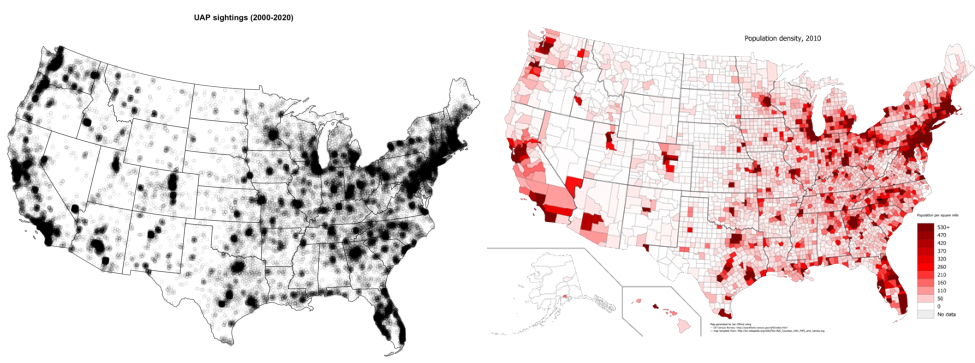
\includegraphics[width=1\linewidth]{lmm_paper_files/figure-latex/unnamed-chunk-1-1} \caption{Right: Plot of UAP sightings from 2000--2020 (by author, from NUFORC database). Left: Plot of population density (U.S. Census). The two maps portray the same latent factor: population density.}\label{fig:unnamed-chunk-1}
\end{figure}

Although no previous works take a similar approach as this paper, a
number of studies have investigated the relationship between UAP
sightings, population, population density, land area, etc. Plaza (2015)
comprehensively reviews the historical literature. However, fifteen of
seventeen studies reviewed were written in the previous century, before
the popular use of information technology. Most use smaller data sets
that may no longer exist, and are often limited to smaller European
countries. These studies also rely on univariate analyses, calculations
of averages and correlation coefficients. Finally, many of these studies
were published in obscure journals and are generally unavailable to
modern researchers. Laurent, et al.~(2015) is the only paper using
`modern' statistical methods the author was able to locate. They are
able to corroborate the long-hypothesized relationship between nuclear
sites and UAP, using spatial point pattern analysis on a database of
French reports. They also find a positive relationship between
population density and reports.

This paper proceeds by introducing the notion of \emph{observational
capacity} as the theoretical framework for the subsequent data analysis.
The quantity of UAP observed in a territory is a function of both the
territory's land area and population density. The data set collected for
this project is then described. The next section introduces the linear
mixed effects model, and then provides the results. The final section
concludes the paper. Appendices provide analysis of the model residuals,
as well as an examination of the state of Utah.

\hypertarget{observational-capacity}{%
\section{Observational capacity}\label{observational-capacity}}

Figure 1 makes clear that population is strongly associated with UAP
observations in a given territory. Intuitively, a larger population
means there are more people potentially observing UAP, thus increasing
the probability of reports. Conversely, a smaller population implies
fewer reports.

However, the size of the territory over which the population is spread
must also be considered. Higher population density may create a
duplication of efforts, with multiple observers `covering' the same
portion of the sky simultaneously. This should result in increased
probability of UAP reports. On the other hand, when a large area is
sparsely populated, there is no chance of duplicate observation. Figure
2 illustrates each combination of population density and land area.
Clearly, the large area with a dense population has the best probability
of observing UAPs, while the smaller area with limited population
density has the least.

However, a territory of a given size must have a \emph{saturation
point}, where any increase in population does not lead to an increase in
observations. That is, any additional population observes a portion of
the sky that is already `covered' by many other observers. The
additional observer does not add any additional observational capacity.
The magnitude of the saturation point is directly dependent on the size
of the territory. Larger territories can accommodate more population
before the saturation point is reached. This implies a logarithmic
relationship between population density and observed UAP.

The exact nature of the relationship between area, population, and
probability of UAP sighting can be estimated empirically via statistical
modeling. However, such a model naturally makes a number of assumptions
that are unlikely to hold in reality. For instance, such a model assumes
that every person in a given territory has an equal chance of observing
UAP. In reality, we know that this is not true: An airplane pilot has a
greater chance of observation than a coal miner. The model additionally
assumes that every square meter within a territory has an equal chance
of `manifesting' UAP. As research by Laurent, et al.~(2015) shows, areas
with certain features like a nuclear reactor or a military base seem to
have a higher probability of `attracting' UAP than others. Finally, the
model assumes that rates of reporting do not vary across populations,
that the percent of those who observe UAP that go on to actually file
report it is constant across the United States. Despite these issues,
the model appears to explain UAP observations well enough to serve as a
baseline for future work.

\begin{figure}
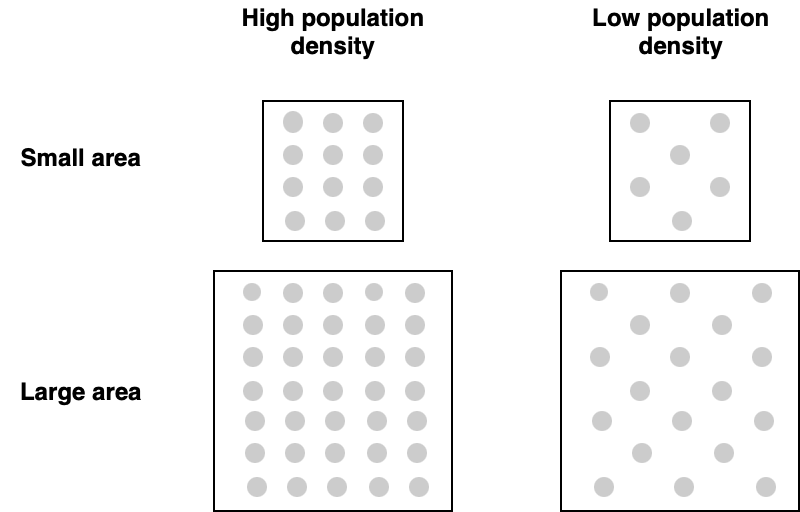
\includegraphics[width=1\linewidth]{./img/diag} \caption{Illustration of population density and area, where each dot represents a unit of population. Larger area or larger density increases the probability of sighting UAP, up to a point where the marginal increase drops to zero sightings.}\label{fig:unnamed-chunk-2}
\end{figure}

\hypertarget{data}{%
\section{Data}\label{data}}

The National UFO Reporting Center was founded in 1974. Since then, it
has collected tens of thousands of sightings. Reports were initially
collected by a 24-hour telephone hotline, but can now be made via the
Internet. They are processed by NUFORC staff, and then uploaded to a
public website. Staff sometimes annotate reports, such as sightings of
obvious man-made satellites. The standard entry provides an account of
the event by the witness, the date and location, the object's shape, and
the duration of sighting.

Renner (2017) provides Python code to scrape these reports from the
NUFORC web site, and compile them into a central data file. The reports
undergo a series of automatic cleaning and standardization, including
using the free GeoLite2 geolocation database (Maxmind). Additional
processing by this author includes removing records marked as obvious
satellites, labeling all five boroughs of New York City as `New York
City', etc.

A total of 55,282 sighting records remain. All 48 continental states are
well-represented, including nearly 10 thousand cities and towns, across
2500 counties. All large- and medium-sized cities are present. The top
10 cities are listed in table 1. Several of America's most populous
cities are included. Figure 3 demonstrates substantial variation in
reports over time. Reports peaked in 2014 near 7 thousand, rapidly
declined to under 3 thousand in 2018, and then swing upward in the final
two years of the decade.

\begin{longtable}[]{@{}llr@{}}
\caption{Cities with most UAP reports.}\tabularnewline
\toprule
state & city & reports \\
\midrule
\endfirsthead
\toprule
state & city & reports \\
\midrule
\endhead
AZ & Phoenix & 328 \\
NY & New York & 327 \\
NV & Las Vegas & 324 \\
WA & Seattle & 278 \\
OR & Portland & 277 \\
CA & San Diego & 228 \\
FL & Orlando & 227 \\
NM & Albuquerque & 224 \\
AZ & Tucson & 210 \\
CA & Los Angeles & 207 \\
\bottomrule
\end{longtable}

\begin{figure}

{\centering 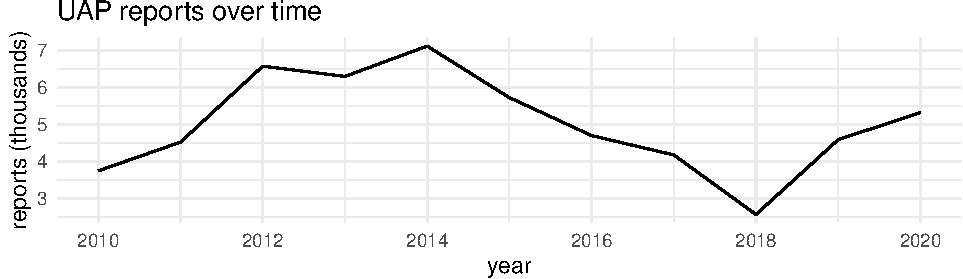
\includegraphics[width=1\linewidth]{lmm_paper_files/figure-latex/unnamed-chunk-5-1} 

}

\caption{Total UAP reports per year.}\label{fig:unnamed-chunk-5}
\end{figure}

Data for the explanatory variables, population and land area, were
retrieved from the U.S. Census. The best and most granular data was
available at the county-level. This necessitated mapping the number of
UAP sightings from city- to county-level. Census indexes were essential
for this conversion. The unit of analysis for the rest of this paper is
thus county-year.

The Census (2021) provides yearly population and population density from
2010--2020 for every county. This data was accessed painlessly via the
\texttt{tidycensus} R package (Walker, et al., 2021). The land area
(square miles) of each U.S. county is available as of 2010, but not
annually. However, it seems to reasonable to assume most counties' land
area do not change substantially from year-to-year.

Figure 4 shows the distributions of and relationships between each of
the variables. The decimal numbers refer to the Pearson correlation
between two variables. The number of asterisks indicate the statistical
significance of the correlation, with more indicating a smaller
\(p\)-value. The bottom plot shows the relationships after a logarithmic
transformation of each variable. The linearity of each relationships
strengthens considerably. Therefore each variable is log-transformed
before modeling.

\begin{figure}

{\centering 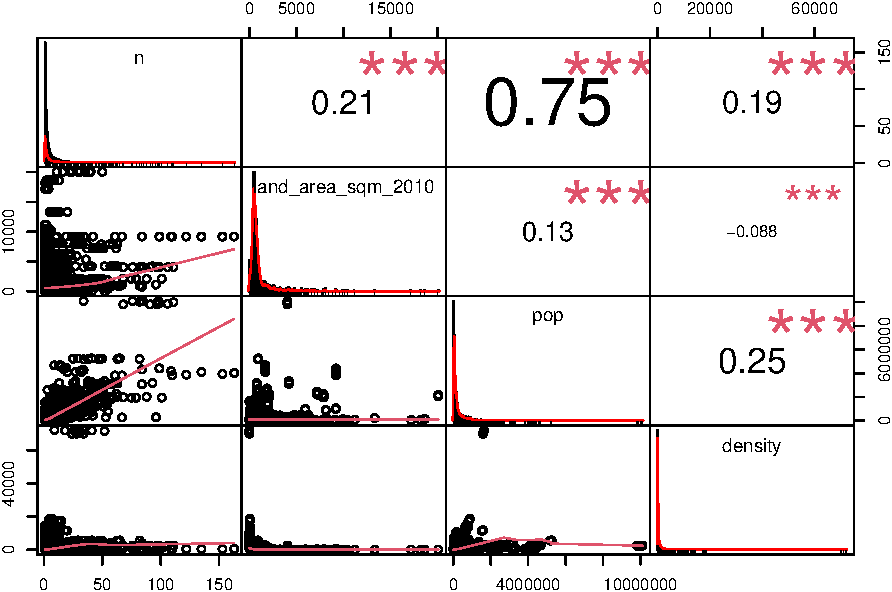
\includegraphics[width=1\linewidth]{lmm_paper_files/figure-latex/unnamed-chunk-6-1} 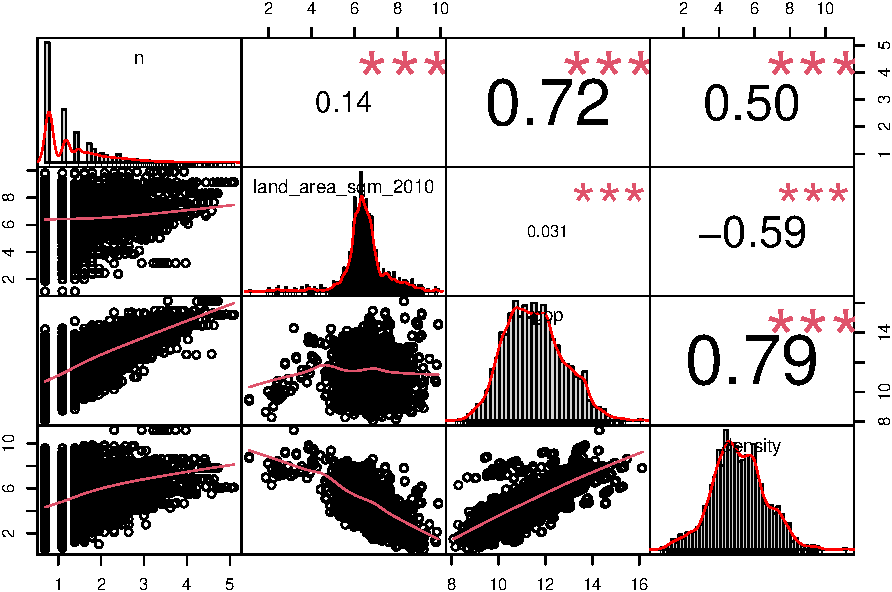
\includegraphics[width=1\linewidth]{lmm_paper_files/figure-latex/unnamed-chunk-6-2} 

}

\caption{Top: Distributions of and relationships between all variables. Bottom: Same, but log-transformed.}\label{fig:unnamed-chunk-6}
\end{figure}

\hypertarget{model}{%
\section{Model}\label{model}}

The association between number of sightings and the independent
variables is modeled using mixed effects linear regression (Gelman and
Hill 2006; Galecki and Burzykowski 2013). For each individual county
\(i\) in year \(j\), the number of UAP reports \(y_{ij}\) is modeled
using regression, with land areaas \(x_{1i}\), and population density as
\(x_{2ij}\). Because of the longitudinal nature of the data, random
slope effects are included for year \(\gamma_j\) and for county
\(\alpha_i\). Both are normally distributed around zero with a standard
deviation \(\sigma^2\):

\[y_{ij} = \mu + \beta_1 x_{1i} + \beta_2 x_{2ij} + \beta_3 x_{1i} x_{2ij} + \alpha_i + \gamma_j + \epsilon_{i}\]
where:

\begin{itemize}
\tightlist
\item
  \(\mu\) is the intercept term, representing overall mean number of
  sightings
\item
  \(\alpha_i \sim N(0,~ \sigma^2_{\alpha})\) is the `effect' of the
  county \(i\)
\item
  \(\gamma_j \sim N(0,~ \sigma^2_{\gamma})\) is the `effect' of the year
  \(j\)
\end{itemize}

The dependent variable is logged, whereas the two independent variables
have been logged and standardized (omitted in the notation above for
clarity's sake). Additionally, an intercept term is included, to test
the possibility that the effect of population density varies depending
on land area, and vice versa. Parameters are estimated to maximize the
log-likelihood of the data, using R's \texttt{lmer4} package (Bates, et
al., 2007). The estimated parameters are given in table 2. As always,
the reader should not interpret regression results as suggesting a
causal relationship, but only a statistical association.

\begin{table}[!htbp] \centering 
  \caption{Estimated model parameters} 
  \label{} 
\begin{tabular}{@{\extracolsep{5pt}}lc}
\\[-1.8ex]\hline 
\hline \\[-1.8ex] 
 & \multicolumn{1}{c}{\textit{Dependent variable:}} \\ 
\cline{2-2} 
\\[-1.8ex] & \multicolumn{1}{c}{n} \\ 
\hline \\[-1.8ex] 
 land\_area\_sqm\_2010 & $0.558^{***}$ \\ 
  & (0.012) \\ 
  & \\ 
 density & $0.481^{***}$ \\ 
  & (0.007) \\ 
  & \\ 
 land\_area\_sqm\_2010:density & $-0.027^{***}$ \\ 
  & (0.004) \\ 
  & \\ 
 Constant & $0.783^{***}$ \\ 
  & (0.048) \\ 
  & \\ 
\hline \\[-1.8ex] 
Observations & \multicolumn{1}{c}{11,785} \\ 
Log Likelihood & \multicolumn{1}{c}{-9,823.979} \\ 
Akaike Inf. Crit. & \multicolumn{1}{c}{19,661.960} \\ 
Bayesian Inf. Crit. & \multicolumn{1}{c}{19,713.580} \\ 
Conditional $R^2$ & \multicolumn{1}{c}{0.673} \\ 
Marginal $R^2$ & \multicolumn{1}{c}{0.484} \\ 
\hline 
\hline \\[-1.8ex] 
\textit{Note:}  & \multicolumn{1}{r}{$^{*}$p$<$0.1; $^{**}$p$<$0.05; $^{***}$p$<$0.01} \\
\end{tabular} 
\end{table}

All variables, including the interaction term, are highly significant. A
comprehensive analysis of model residuals indicates that the model meets
the assumptions of linear regression (but see the appendix).

The interaction term necessarily implies that the association between
density and the number of UAP observations varies according to the size
of the land area, and vice versa Thus a graphical display communicates
the model most succinctly:

\begin{figure}

{\centering 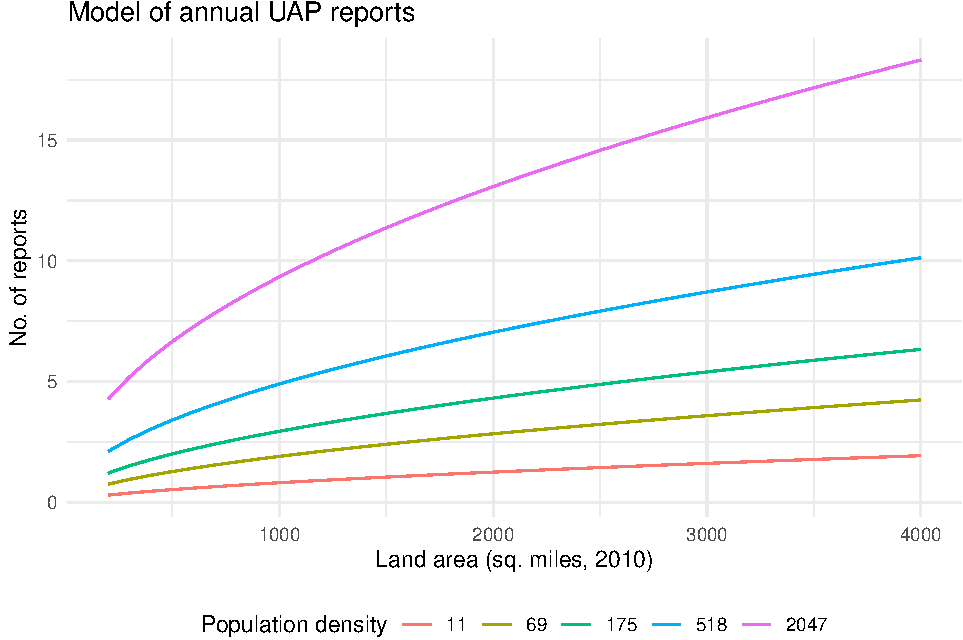
\includegraphics[width=1\linewidth]{lmm_paper_files/figure-latex/unnamed-chunk-8-1} 

}

\caption{Graphical display of fit model.}\label{fig:unnamed-chunk-8}
\end{figure}

This plot shows how the number of annual UAP sightings in a `generic'
county varies by land area area and population density. At low
population density (red), the number of sightings increases very slowly
even as land area quadruples. Observational capacity does not increase
quickly. In contrast, at high population density (purple), sightings
increase much faster as land area increases. For all levels of
population density, however, there is a point where the rate of increase
of sightings declines.

\hypertarget{results-and-discussion}{%
\section{Results and discussion}\label{results-and-discussion}}

The section begins by examining the random slope parameters estimated
for each county \(\hat{\alpha}_i\). These values represent the annual
`effect' of each particular county, over and above the effects of
population and area.

Table 3 below displays the top estimates, multiplied by ten to show how
many excess sightings are observed over the entire decade-long data set.

\begin{longtable}[]{@{}lllr@{}}
\caption{Excess sightings by county.}\tabularnewline
\toprule
State & County & Largest city & Excess sightings \\
\midrule
\endfirsthead
\toprule
State & County & Largest city & Excess sightings \\
\midrule
\endhead
S. Carolina & Horry & Myrtle Beach & 54 \\
Arizona & Maricopa & Phoenix & 48 \\
Washington & King & Seattle & 46 \\
Idaho & Ada & Boise & 39 \\
Oregon & Multnomah & Portland & 35 \\
California & San Diego & San Diego & 33 \\
Washington & Snohomish & Everett & 33 \\
California & Los Angeles & Los Angeles & 33 \\
California & Riverside & Riverside & 30 \\
Washington & Clark & Vancouver & 30 \\
\bottomrule
\end{longtable}

Even allowing for these adjustments, some counties record far higher
sightings than expected. For instance, Maricopa county has 1137
sightings, whereas the model predicts only 784. For the most part, the
excess is attributable to handful of years only. In Maricopa's case,
these are the years 2014--15, the global peak of sightings. The table 4
below shows the largest model errors at the unit-level. For the most
part, they are clustered around this peak, with Horry and Maricopa
counties dominating the list.

\pagebreak

\begin{longtable}[]{@{}rllrrr@{}}
\caption{Largest model errors, by year-county.}\tabularnewline
\toprule
year & state & county\_name & n & pred & error \\
\midrule
\endfirsthead
\toprule
year & state & county\_name & n & pred & error \\
\midrule
\endhead
2015 & Arizona & Maricopa & 163 & 76 & 87 \\
2014 & South Carolina & Horry & 96 & 25 & 71 \\
2014 & Arizona & Maricopa & 153 & 87 & 66 \\
2016 & Arizona & Maricopa & 135 & 69 & 66 \\
2012 & Washington & King & 101 & 51 & 50 \\
2017 & Arizona & Maricopa & 109 & 64 & 45 \\
2012 & South Carolina & Horry & 67 & 23 & 44 \\
2014 & California & Orange & 84 & 41 & 43 \\
2014 & California & San Diego & 93 & 51 & 42 \\
2013 & Arizona & Maricopa & 122 & 82 & 40 \\
\bottomrule
\end{longtable}

Previous work have tried to `control for' the effects of population by
putting sightings into a per capita number (described in Plaza 2015).
This calculation is duplicated below in table 5. The top ten list is
substantially different than what is given by the mixed effects model;
only Horry county is shared between them. Simply dividing by population
does not fully account for effects of population. Additionally, it is
less practically useful---it does not make sense to place expensive
instrumentation in a territory that sees less than one sighting per
year!

\begin{longtable}[]{@{}llrrr@{}}
\caption{Top counties by per capita UAP reports. This ordering is
substantially different compared to the model, and less practically
useful.}\tabularnewline
\toprule
state & county\_name & mean\_pop & n & per\_capita\_year \\
\midrule
\endfirsthead
\toprule
state & county\_name & mean\_pop & n & per\_capita\_year \\
\midrule
\endhead
South Carolina & Horry & 296253 & 385 & 0 \\
Virginia & Fredericksburg & 27012 & 35 & 0 \\
Oregon & Lincoln & 46867 & 60 & 0 \\
Oregon & Clatsop & 37786 & 44 & 0 \\
Texas & La Salle & 6922 & 8 & 0 \\
North Carolina & Dare & 34722 & 40 & 0 \\
Kansas & Thomas & 7906 & 8 & 0 \\
South Carolina & Georgetown & 60942 & 60 & 0 \\
New Mexico & Taos & 32867 & 32 & 0 \\
Arizona & La Paz & 20611 & 20 & 0 \\
\bottomrule
\end{longtable}

The mixed effects model helps us to `look past' the effects of
population and land area, to more clearly identify unusually active
areas. However, it does not explain \emph{why} these areas are
especially active. The model identifies areas worthy of additional study
only. For instance, a county may have an unusual number of sightings
because a single resident is a UFO obsessive, relentlessly reporting
every object in the sky. The NUFROC database entries do not offer an
anonymized user ID that would help identify such entries. Additionally,
a city may have an active UFO group, creating a higher reporting rate
than other locations. The locale's culture around UAP may also influence
the number of reports. This may be the case with the most anomalous city
identified by the model, Myrtle Beach. At one point, Myrtle Beach hosted
a UFO/alien museum called Encounters: UFO Experience, very close to the
beach (TripAdvisor). This may have put visitors into the mindset where
they are more likely to identify common sights as anomalous, then seek
out a venue to report them.

Given the stereotypical UFO experience occurs in a remote region, far
from large concentrations of people, it may seem odd that reports should
be positively associated with population. Indeed, computer scientist
Jacques Valleé has gone so far as to promulgate a `law': UFO landings
are inversely correlated with population density (Valleé 1966). However,
the vast majority of records in the NUFROC data concern \emph{sightings
in the sky}, and not landings or so-called `high strangeness.' Plaza
(2015) shows that there is no contradiction between this `law' and the
model fit above. Indeed, this paper largely supports Plaza's findings.

\hypertarget{conclusion}{%
\section{Conclusion}\label{conclusion}}

Mapping UAP observations from large sightings databases may seem like a
promising way to begin investigation, but it is stymied by the
overwhelming effect of population. This paper developed a simple mixed
effects regression model to account for this effect. By modeling a
county's number of sightings as a function of land area and population
density, it is possible to produce a superior list of potential UAP `hot
spots.' Among the leading hot spots include Myrtle Beach (SC), Phoenix
(AR), and Seattle (WA). This list can be used to generate future
hypotheses to test. It may also suggest optimal placements for
electronic sensor platforms. Additional work extending this model may
bring us closer to a scientific explanation for the UAP mystery.

\pagebreak

\hypertarget{appendix-model-diagnostics}{%
\section{Appendix: Model diagnostics}\label{appendix-model-diagnostics}}

Model residuals are normally distributed, including those for the random
effects of year and county. Collinearity is not an issue. It does appear
that county-years with only a few sightings, and county-years with many
sightings, have a mean residual greater than zero. This indicates the
model has higher rates for low population areas with few sightings, as
well very large territories. The latter represent the `excess sightings'
this paper has tried to identify. Residuals do not appear to vary with
either of the independent variables. Random slopes are confirmed as
approximately normally distributed.

\begin{figure}

{\centering 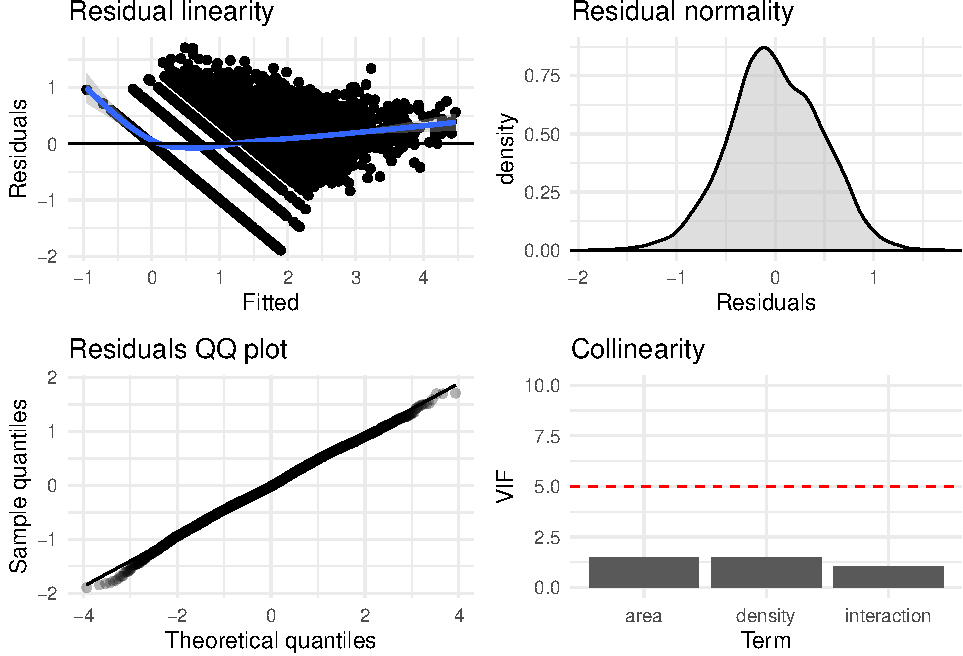
\includegraphics[width=1\linewidth]{lmm_paper_files/figure-latex/unnamed-chunk-11-1} 

}

\caption{Diagnostics of model show the model mostly meets the conditions for valid inference.}\label{fig:unnamed-chunk-11}
\end{figure}

\pagebreak

\hypertarget{appendix-utah}{%
\section{Appendix: Utah}\label{appendix-utah}}

Utah is often considered an area of concentrated UAP (Salisbury 2010).
Because of this reputation, it is worth examining more closely. After
accounting for area and population, the top Utah hot spots are:

\begin{longtable}[]{@{}llrrr@{}}
\caption{Utah counties with highest number of sightings.}\tabularnewline
\toprule
state & county\_name & n & pred & excess \\
\midrule
\endfirsthead
\toprule
state & county\_name & n & pred & excess \\
\midrule
\endhead
Utah & Salt Lake & 256 & 196 & -60 \\
Utah & Utah & 118 & 98 & -20 \\
Utah & Davis & 60 & 55 & -5 \\
Utah & Weber & 34 & 30 & -4 \\
Utah & Washington & 31 & 28 & -3 \\
Utah & Tooele & 17 & 16 & -1 \\
Utah & Cache & 15 & 14 & -1 \\
Utah & Iron & 14 & 13 & -1 \\
Utah & Summit & 13 & 12 & -1 \\
Utah & Box Elder & 10 & 10 & 0 \\
Utah & Uintah & 9 & 9 & 0 \\
\bottomrule
\end{longtable}

Salt Lake City clearly dominates the list as Utah's greatest hot spot,
even after accounting for population and area. Utah county also
manifests excessive UAP, although the rest of Utah appears to be in line
with expectations.

Uintah county, a notable hot spot, has the eleventh-most sightings in
Utah. Its nine reported sightings from 2010--2020 perfectly matches the
model's predictions. This is unusual because of the area's reputation
for reports of bizarre phenomena. However, this may not be as puzzling
as it seems. As Salisbury noted, `Incidentally, the people of the Uintah
Basin didn't bother to report their sightings to the authorities,'
instead reporting them to a local science teacher by the name of Junior
Hicks (2010, 28).

\pagebreak

\hypertarget{references}{%
\section{References}\label{references}}

\setlength{\parindent}{-0.25in}
\setlength{\leftskip}{0.25in}
\setlength{\parskip}{6pt}

Bates, Douglas, Martin Maechler, Ben Bolker, et al.~2007. `The
\texttt{lme4} package.' R package.

Cooper, Helene, Ralph Blumenthal, and Leslie Kean. 2017. ``Glowing auras
and `black money': The Pentagon's mysterious UFO program.'' \emph{New
York Times}, Dec.~16.

David, Leonard. 2021. `Spotting UFOs: Do-it-yourself sky surveillance
comes online.' \emph{Space.com}, March 3.
\textless{}\texttt{https://www.space.com/spotting-ufos-sky-}
\texttt{hub-surveillance}\textgreater.

Gałecki, Andrzej, and Tomasz Burzykowski. 2013. \emph{Linear
Mixed-Effects Models Using R: A Step-By-Step Approach} (Springer).

Gelman, Andrew, and Jennifer Hill. 2006. \emph{Data Analysis Using
Regression and Multilevel/Hierarchical Models} (Cambridge University
Press).

Laurent, Thibault, Christine Thomas-Agnan, and Michaël Vaillant. 2015.
`Spatial point pattern analysis of the Unidentified Aerial Phenomena in
France.' \emph{arXiv} preprint \texttt{1509.00571}.

Loeb, Avi. 2021. `Announcing a new plan for solving the mystery of
unidentified aeriel phenomena.' \emph{Scientific American}, July 26.\\
\textless{}\texttt{https://www.scientificamerican.com/article/announcing-a-new-plan-}
\texttt{for-solving-the-mystery-of-unidentified-aerial-phenomena/}\textgreater.

Maxmind. Geolite2 geolocation database.
\textless{}\texttt{https://dev.maxmind.com/geoip/}
\texttt{geolite2-free-geolocation-data}\textgreater.

ODNI (Office of the Director of National Intelligence). 2021.
`Preliminary Assessment: Unidentified Aerial Phenomena.' June 25.
\textless{}\texttt{https://www.dni.gov/}
\texttt{files/ODNI/documents/assessments/Prelimary-Assessment-UAP-}
\texttt{20210625.pdf}\textgreater.

Plaza, Julio. 2015. `A review on the relation between population density
and UFO sightings.' \emph{Journal of Scientific Exploration} 29, no. 3:
425--48.

R Core Team. 2020. R: A Language and Environment For Statistical
Computing. R Foundation for Statistical Computing, Vienna, Austria.\\
\textless{}\texttt{https://www.R-project.org/}\textgreater.

Renner, Timothy. 2017. `NUFORC Sighting Reports.' Github repository.
\textless{}\texttt{https://github.com/timothyrenner/nuforc\_sightings\_data/}\textgreater.

Salisbury, Frank B. 2010. \emph{The Utah UFO Display: A Scientist's
Report} (Cedar Fort).

TripAdvisor. `Things to do in Myrtle Beach: Encounters UFO Experience.'
\textless{}\texttt{https://www.tripadvisor.com/Attraction\_Review-g54359-d4145792-}\\
\texttt{Reviews-Encounters\_UFO\_Experience-Myrtle\_Beach\_South\_Carolina.html}\textgreater.

U.S. Census Bureau. 2011. Land area: Excel file \texttt{LND01.xls}.
\emph{Statistical Abstract of the United States}. Available at
\textless{}\texttt{https://www.census.gov/library/}
\texttt{publications/2011/compendia/usa-counties-2011.html}\textgreater.

U.S. Census Bureau. 2020. Gazatteer Files. Available at
\textless{}\texttt{https://www.\ census.gov/geographies/reference-files/time-series/geo/gazetteer-}
\texttt{files.html}\textgreater.

Valleé, Jacques. 1966. `The patterns behind the UFO landings.'
\emph{Flying Saucer Review} no. 1: 8--27. Available at
\textless{}\texttt{http://www.ignaciodarnaude.com/ufologia/}
\texttt{Vallee,Pattern\%20behind\%20UFO\%20landings,FSR-SI\%201966\%20N\%201,}
\texttt{Humanoids.pdf}\textgreater.

Walker, Kyle, Matt Herman, and Kris Eberwein. 2021. \texttt{tidycensus}.
R package.
\textless{}\texttt{https://cran.r-project.org/web/packages/tidycensus/}\textgreater.


\end{document}
